\subsection{Distribuição da Ação $Mover(r)$}\label{subsec:distr_mov}

Para gerar as ações do tipo $Mover(r)$, são utilizadas três distribuições
uniformes circulares, conforme apresentado na Figura~\ref{fig:distr_mov}. Esta
distribuição é centrada em cada robô.

\begin{figure}[H]
  \centering
  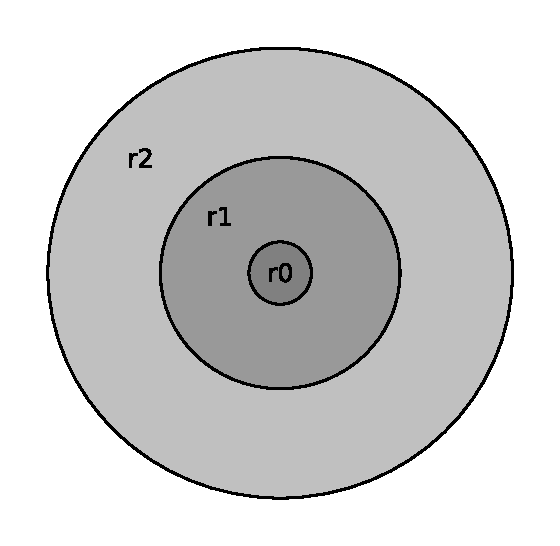
\includegraphics[width=0.5\linewidth] {distr_mov}
  \caption{Distribuição da Ação $Mover(r)$}\label{fig:distr_mov}
\end{figure}

% vim: tw=80 et ts=2 sw=2 sts=2 ft=tex
